\begin{pastexam}[label={px:gk3-109-ds-02}]{高考三級資訊處理 109 年 第二題}
（申論；30 分）

優先佇列（Priority Queue）是依管理物件的優先權來考量，在此我們考慮管理物件的鍵值（Key）愈小其優先
權愈高，兩個主要操作則分別為加入（Insert）與擷取最小者（Delete\_Min）。
\begin{itemize}[leftmargin=2em, labelsep=0.3em, itemsep=2pt]
\item[㈠] 請說明如何利用優先佇列對 $n$ 個鍵值進行排序。（6 分）
\item[㈡] 我們使用一個未排序的陣列（Unsorted Array）來管理鍵值以實現一個優先佇列，請回答下列問題：
（10 分）
\begin{itemize}[leftmargin=2em, labelsep=0.3em, itemsep=1pt]
\item[⑴] 若有 $n$ 個鍵值，請說明兩個主要操作（加入（Insert）與擷取最小者（Delete\_Min））的時間
複雜度。
\item[⑵] 請判斷下面的敘述是否為真，並請說明原因：若以此優先佇列進行排序（Sorting），其所對應的
排序原理為插入排序（Insertion Sort）。
\end{itemize}
\item[㈢] 二元堆積（Binary Heap）是一個優先佇列的資料結構，因為我們考慮鍵值小的物件有高的優先權，
所以又可稱為最小堆積（Minimum Heap）。（14 分）
\begin{itemize}[leftmargin=2em, labelsep=0.3em, itemsep=1pt]
\item[⑴] 在結構上最小堆積為一個完全二元樹（Complete Binary Tree），若使用一個陣列來實作最小堆積，
陣列中物件的鍵值放置如下，請描述此陣列對應的完全二元樹（以樹狀結構表示）。
\begin{center}
\begin{tabular}{|c|c|c|c|c|c|c|c|c|c|c|}
\hline
Index & 1 & 2 & 3 & 4 & 5 & 6 & 7 & 8 & 9 & 10 \\ \hline
Key & 35 & 18 & 42 & 24 & 7 & 14 & 25 & 12 & 38 & 21 \\ \hline
\end{tabular}
\end{center}
\item[⑵] 請說明二元堆積中何謂堆積特性（Heap Property）？
\item[⑶] 前揭⑴中的完全二元樹並未有堆積特性，請將其進行堆積化（Heapify），並以陣列表示出堆積
化後的最小堆積所對應之完全二元樹。
\end{itemize}
\end{itemize}
\end{pastexam}

\begin{pastsoln}

\textbf{㈠ 用優先佇列排序}：先把 $n$ 個鍵值逐一 Insert 進優先佇列，再連續做 $n$ 次 Delete\_Min，
依序取出的就是由小到大的順序（每次取出的都是剩下的最小值）。
\begin{pseudo}{用優先佇列排序}
\Procedure{PQ-Sort}{$A, n$}
    \State $Q \gets$ 空的優先佇列
    \For{$i \gets 1$ \To $n$}
        \State \Call{Insert}{$Q, A[i]$}
    \EndFor
    \For{$i \gets 1$ \To $n$}
        \State $A[i] \gets$ \Call{Delete\_Min}{$Q$}
    \EndFor
\EndProcedure
\end{pseudo}
總時間 $= n \cdot (\text{Insert 的時間}) + n \cdot (\text{Delete\_Min 的時間})$。 用二元堆積時兩者都
$O(\lg n)$，總共 $O(n \lg n)$，這就是堆積排序（資結書第~14.6~節）。

\textbf{㈡⑴} 未排序陣列 $A[1..m]$（$m$ 是目前的個數，最多 $n$）：
\begin{itemize}[nosep]
\item \textbf{Insert}：直接放在最後，$A[m+1] \gets x$，$m \gets m + 1$，$O(1)$。
\item \textbf{Delete\_Min}：最小值可能在任何位置，要掃描全部 $m$ 個找出最小的（$m - 1$ 次比較），
再把最後一個搬到它的位置填洞、$m \gets m - 1$，$\Theta(m) = O(n)$。
\end{itemize}

\textbf{㈡⑵ 敘述為假。} 依㈠，$n$ 次 Insert 只是把資料原樣放進陣列；排序的工作全在 Delete\_Min：
每次在「還沒取出的數」裡掃描找最小值、把它取出，第 $i$ 次比較 $n - i$ 次，共 $n(n-1)/2$ 次。
這正是\textbf{選擇排序}（selection sort）的原理：每一輪從未排序的部分\textbf{選出}最小的放到已排序部分
的尾端（資結書虛擬碼~14.2）。 插入排序則是每次拿下一個數，\textbf{插入}已排序部分的正確位置，
對應的是用\textbf{已排序陣列}實作的優先佇列：Insert 時要找位置、搬移，$O(n)$；Delete\_Min 只要取
最前面（或最後面）那個，$O(1)$。 兩種實作做排序都是 $\Theta(n^2)$，但對應的排序法不同。

\textbf{㈢⑴} 節點 $i$ 的左子是 $2i$、右子是 $2i + 1$。 所以 $35$ 是根；$18$、$42$ 是它的子節點；
$18$ 的子節點是 $24$、$7$；$42$ 的子節點是 $14$、$25$；$24$ 的子節點是 $12$、$38$；$7$ 的左子是
$21$。
\begin{center}
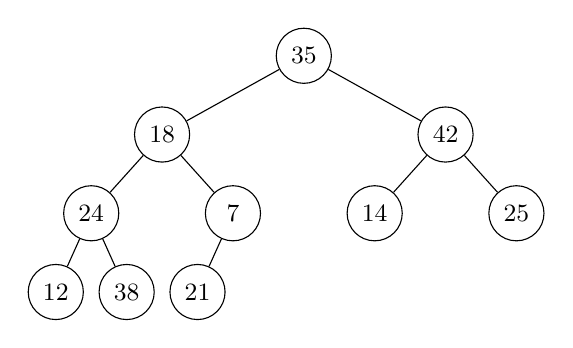
\begin{tikzpicture}[level distance=10mm,
  level 1/.style={sibling distance=36mm}, level 2/.style={sibling distance=18mm},
  level 3/.style={sibling distance=9mm},
  every node/.style={circle, draw, minimum size=7mm, inner sep=0pt, font=\small}]
\node {35}
  child {node {18} child {node {24} child {node {12}} child {node {38}}}
                   child {node {7} child {node {21}} child[missing]}}
  child {node {42} child {node {14}} child {node {25}}};
\end{tikzpicture}
\end{center}

\textbf{㈢⑵ 堆積特性}（最小堆積）：每個節點的鍵值都不大於它的子節點的鍵值，用陣列寫就是
$A[\lfloor i/2 \rfloor] \le A[i]$，$2 \le i \le n$。 因此根 $A[1]$ 是最小值；但兄弟之間、左右
子樹之間沒有大小規定。 加上「完全二元樹」這個形狀條件，才是二元堆積。 ⑴的樹不滿足，例如根
$35 > 18$。

\textbf{㈢⑶ 堆積化}：用由下而上的建堆積（資結書第~8.2~節）：從最後一個有子節點的節點
$\lfloor 10/2 \rfloor = 5$ 開始，往前到根，對每個節點做「往下調整」：和較小的子節點比，子節點較小就
交換，一路往下直到不必換。
\begin{center}
\small
\begin{tabular}{cp{5.6cm}l}
\toprule
節點 & 動作 & 之後的陣列 $A[1..10]$ \\
\midrule
5（7） & 子節點 21，$7 < 21$，不動 & 35, 18, 42, 24, 7, 14, 25, 12, 38, 21 \\
4（24） & 子節點 12、38，和 12 換 & 35, 18, 42, \textbf{12}, 7, 14, 25, \textbf{24}, 38, 21 \\
3（42） & 子節點 14、25，和 14 換 & 35, 18, \textbf{14}, 12, 7, \textbf{42}, 25, 24, 38, 21 \\
2（18） & 子節點 12、7，和 7 換；到節點 5，子節點 21 比 18 大，停 & 35, \textbf{7}, 14, 12, \textbf{18}, 42, 25, 24, 38, 21 \\
1（35） & 和 7 換；到節點 2，子節點 12、18，和 12 換；到節點 4，子節點 24、38，和 24 換；到節點 8，葉，停 & \textbf{7}, \textbf{12}, 14, \textbf{24}, 18, 42, 25, \textbf{35}, 38, 21 \\
\bottomrule
\end{tabular}
\end{center}
堆積化後的陣列：
\begin{center}
\begin{tabular}{|c|c|c|c|c|c|c|c|c|c|c|}
\hline
Index & 1 & 2 & 3 & 4 & 5 & 6 & 7 & 8 & 9 & 10 \\ \hline
Key & 7 & 12 & 14 & 24 & 18 & 42 & 25 & 35 & 38 & 21 \\ \hline
\end{tabular}
\end{center}
對應的完全二元樹：
\begin{center}
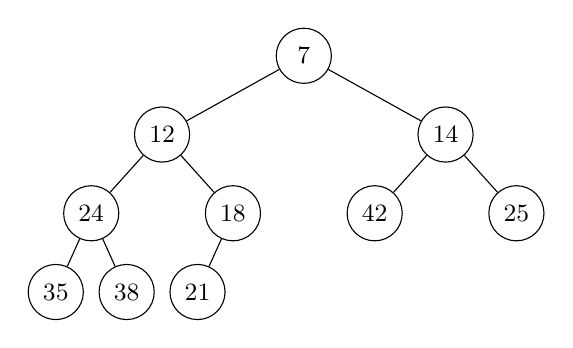
\begin{tikzpicture}[level distance=10mm,
  level 1/.style={sibling distance=36mm}, level 2/.style={sibling distance=18mm},
  level 3/.style={sibling distance=9mm},
  every node/.style={circle, draw, minimum size=7mm, inner sep=0pt, font=\small}]
\node {7}
  child {node {12} child {node {24} child {node {35}} child {node {38}}}
                   child {node {18} child {node {21}} child[missing]}}
  child {node {14} child {node {42}} child {node {25}}};
\end{tikzpicture}
\end{center}
檢查：$7 \le 12, 14$；$12 \le 24, 18$；$14 \le 42, 25$；$24 \le 35, 38$；$18 \le 21$，每個節點都不大於
子節點。 由下而上建堆積的總時間是 $O(n)$（資結書定理~8.1）；若改成把 $10$ 個鍵逐一 Insert，結果的
陣列可能不同，但同樣是合法的最小堆積。
\end{pastsoln}
